%-----------------------------------------------------------------------------%
\chapter{\babLima}
\label{bab:5}

Bab ini membahas mengenai hasil dan analisis dari evaluasi yang telah dilaksanakan berdasarkan skenario-skenario yang telah disusun pada bab sebelumnya. Pembahasan analisis akan dibagikan berdasarkan aspek-aspek yang telah disusun untuk memberikan gambaran yang lebih jelas mengenai performa program dan \textit{resource} atau sumber daya yang dibutuhkan untuk mencapai performa tersebut. Selain itu, bab ini juga akan membahas pertimbangan variasi dari PeerToCP yang lebih baik digunakan dan faktor-faktor yang memengaruhi pertimbangan tersebut. Melalui pertimbangan tersebut, kelemahan dari sistem aplikasi turut disampaikan untuk perkembangan ke depannya.

\section{Aspek \textit{Local-First} dan \textit{Correctness}}

Kedua aspek ini tidak dapat dipisahkan satu sama lain, pada skenario pertama dan kedua, aspek \textit{local-first} diuji dengan mensimulasikan proses pemutusan koneksi secara acak pada klien, sementara data terus diubah oleh setiap pengguna lokal. Berdasarkan eksperimen secara langsung, proses perubahan ini terjadi secara \textit{local-first}, yang berarti perubahan lokal dapat terus dilakukan dan langsung diterapkan meskipun klien sedang tidak berada dalam jaringan, dan ketika terjadi proses masuk kembali ke jaringan, data akan diperbaharui secara sesuai dengan perubahan yang dilakukan.

Berdasarkan eksperimen yang dilakukan, setiap variasi dari PeerToCP menghasilkan nilai cacahan yang sama untuk setiap skenarionya, yang berarti setiap dokumen berada pada kondisi atau \textit{state} akhir yang sama. Namun pada skenario pertama dengan 8 klien pada variasi Operational Transformation yang berbasis \textit{Client-Server}, dapat terjadi pemutusan hubungan \textit{disconnection} yang tidak dapat terhubung kembali karena \textit{bandwidth} koneksi internet yang berada di luar batas \textit{environment} pengujian.

Skenario dengan jumlah klien ini diulang hingga tiga kali eksperimen, dan dalam setiap eksperimen tersebut, satu hingga dua klien tidak dapat terhubung kembali. Pada eksperimen, waktu pemutusan hubungan dilakukan secara acak dalam periode durasi yang sama untuk setiap kliennya seperti yang dijelaskan pada bab sebelumnya. Hal ini ditunjukkan secara lebih detail pada grafik transmisi data yang masuk melalui jaringan pada klien pertama dan klien kedua untuk setiap variasi aplikasi dalam skenario pertama ini.

\begin{figure}
 \centering
 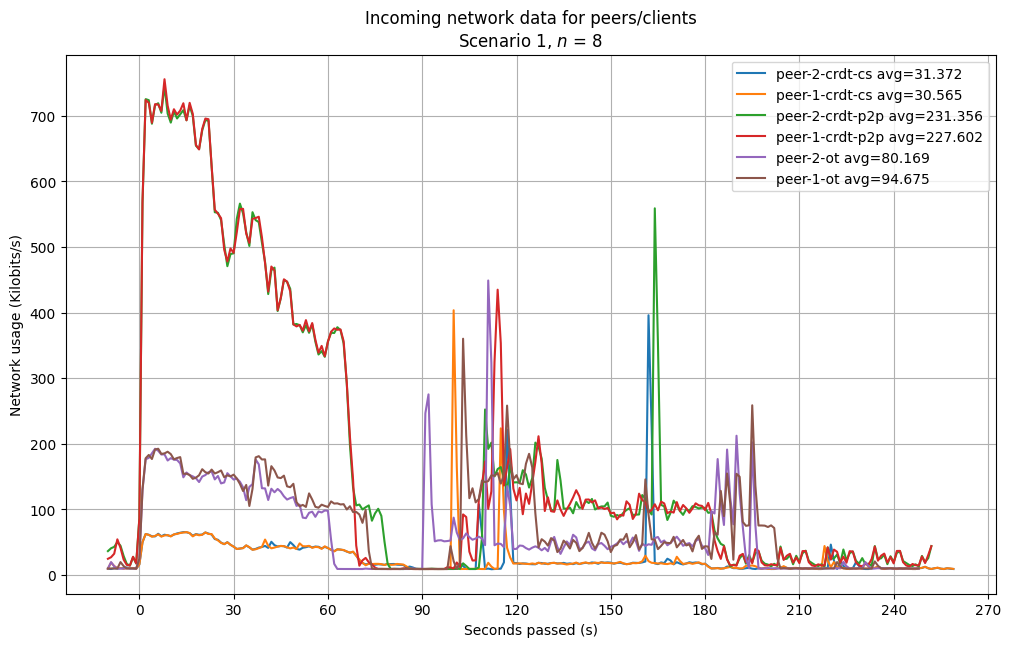
\includegraphics[width=13cm]{./assets/skripsi/benchmark-vis_cell_2_output_23}
 \caption{Grafik Perbandingan Jaringan pada Klien Pertama dan Klien Kedua untuk $n = 8$}
 \label{fig:2-23}
\end{figure}

Pada saat operasi \textit{update} dilakukan tepat setelah koneksi terhubung kembali, ukuran \textit{update} cenderung lebih besar karena sudah terkumpul dari beberapa operasi yang terjadi selama klien sedang berada di luar jaringan. Ketika \textit{update} ini dilakukan, server sedang dalam keadaan berbagai klien lain yang hendak mengirimkan \textit{update}. Karena hal tersebut, algoritma \textit{operational transformation} yang hanya membolehkan suatu \textit{update} untuk dilakukan apabila versi terbaru yang sama sudah dimiliki oleh klien akan meminta klien untuk melakukan \textit{update}. Sementara tumpukan \textit{push update} berukuran besar terus dikirimkan hal ini akan memenuhi \textit{bandwidth} server, yang dapat dilihat pada grafik berikut.

Gambar~\ref{fig:2-23}, menunjukkan klien pertama yang mengalami pemutusan jaringan pada detik ke-72 dan penghubungan kembali pada detik ke-102, terjadi pengiriman data yang cukup besar selama kurang lebih 20 detik. Begitu pula dengan klien kedua yang mengalami pemutusan jaringan pada sekitar detik ke-60 dan penghubungan kembali pada detik ke-90. Sesaat setelah suatu klien terhubung kembali ke suatu jaringan, akan terjadi \textit{spike} pada jaringan yang cukup besar. Pada jumlah pengguna yang cukup banyak dalam satu dokumen, pemutusan dan penghubungan jaringan yang secara sengaja dilakukan pada waktu yang serupa dapat menyebabkan ketidakandalan pada sistem ini. Grafik untuk server ditunjukkan pada gambar berikut.

\begin{figure}
 \centering
 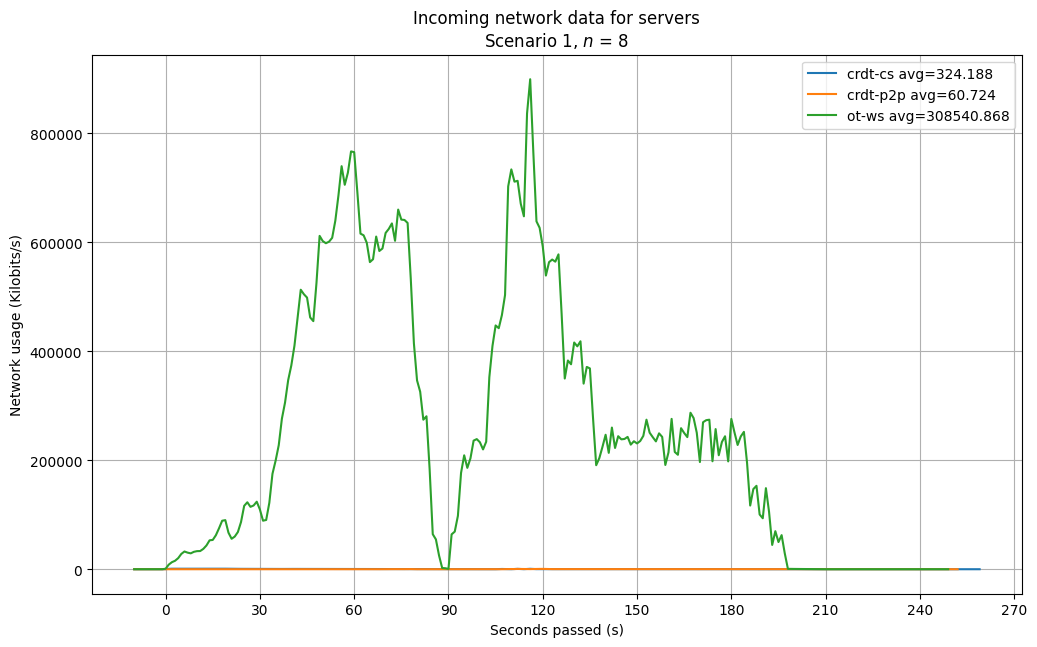
\includegraphics[width=15cm]{./assets/skripsi/benchmark-vis_cell_2_output_24}
 \caption{Grafik Perbandingan Penerimaan Data pada Setiap Variasi Server PeerToCP}
 \label{fig:2-24}
\end{figure}

Lalu lintas jaringan pada server variasi \textit{operational transformation} dengan arsitektur \textit{client-server} dapat mencapai lebih dari 800000 \textit{kilobits}/detik atau setara dengan 100 \textit{megabytes}/detik, sementara untuk skenario yang serupa, transmisi data pada server dengan variasi CRDT berarsitektur \textit{client-server} lebih hemat sekitar 950 kali. Melalui Gambar~\ref{fig:2-24}, diketahui bahwa mean transmisinya sekitar 80 kali lebih sedikit dibandingkan CRDT \textit{peer-to-peer} serta 950 kali lebih sedikit dibandingkan CRDT \textit{client-server}.

Pada skenario pertama ini, terlihat bahwa variasi PeerToCP yang menggunakan CRDT lebih dapat diandalkan karena paralelitas \textit{update} yang dilakukan terhadap dokumen. Faktor-faktor lain yang memengaruhi variasi CRDT yang lebih baik juga tidak menutup kemungkinan dari segi implementasi \textit{provider websocket} yang digunakan, teknik kompresi dan \textit{encoding} yang diterapkan, serta efek bola salju yang ditimbulkan akibat \textit{update} berukuran besar yang terus dikirimkan menjadi tertumpuk dan selalu terlambat dibandingkan \textit{update} lain dan menyangkut aspek selanjutnya yang akan dibahas, yaitu \textit{Scalability} dan \textit{Responsiveness}.

\section{Aspek \textit{Scalability} dan \textit{Responsiveness}}

Latensi dari teks editor secara khusus diukur secara terus menerus pada skenario ketiga tanpa adanya pemutusan hubungan seperti pada skenario pertama dan kedua. Setiap pengguna akan diukur waktu selisih penerimaan datanya terhadap pengguna yang bukan dirinya sendiri dan dicatat latensinya pada waktu data dokumen diterima, kemudian dilakukan rata-rata untuk $n$ pengguna tersebut. Tabel~\ref{tab:latency-3} menunjukkan latensi PeerToCP variasi CRDT \textit{peer-to-peer} memiliki latensi yang paling rendah, namun semakin besar nilai $n$, selisih perbedaan CRDT \textit{client-server} dan CRDT \textit{peer-to-peer} semakin mengecil. Sementara pada variasi OT \textit{client-server}, latensinya dua kali lebih besar dari variasi CRDT \textit{client-server}, dengan lonjakan latensi maksimum hingga dua detik saat $n = 8$.

% Please add the following required packages to your document preamble:
% \usepackage{multirow}
\begin{table}[H]
 \centering
\begin{tabular}{|c|rrr|rrr|rrr|}
\hline
\multirow{2}{*}{$n$} & \multicolumn{3}{c|}{\textbf{CRDT Peer-To-Peer}} & \multicolumn{3}{c|}{\textbf{CRDT Client Server}} & \multicolumn{3}{c|}{\textbf{OT Client Server}} \\ \cline{2-10}
 & \multicolumn{1}{c|}{Mean} & \multicolumn{1}{c|}{Median} & \multicolumn{1}{c|}{Max} & \multicolumn{1}{c|}{Mean} & \multicolumn{1}{c|}{Median} & \multicolumn{1}{c|}{Max} & \multicolumn{1}{c|}{Mean} & \multicolumn{1}{c|}{Median} & \multicolumn{1}{c|}{Max} \\ \hline
\textbf{2} & \multicolumn{1}{r|}{23.30} & \multicolumn{1}{r|}{21.00} & 76.00 & \multicolumn{1}{r|}{39.50} & \multicolumn{1}{r|}{38.00} & 134.00 & \multicolumn{1}{r|}{87.42} & \multicolumn{1}{r|}{84.00} & 168.00 \\ \hline
\textbf{4} & \multicolumn{1}{r|}{34.00} & \multicolumn{1}{r|}{30.00} & 223.00 & \multicolumn{1}{r|}{46.10} & \multicolumn{1}{r|}{42.00} & 220.00 & \multicolumn{1}{r|}{98.84} & \multicolumn{1}{r|}{86.00} & 1225.00 \\ \hline
\textbf{8} & \multicolumn{1}{r|}{55.56} & \multicolumn{1}{r|}{47.00} & 313.00 & \multicolumn{1}{r|}{63.84} & \multicolumn{1}{r|}{56.00} & 308.00 & \multicolumn{1}{r|}{235.62} & \multicolumn{1}{r|}{151.00} & 2010.00 \\ \hline
\end{tabular}
 \caption{Statistik Latensi Operasi Nonlokal pada Skenario Ketiga (Teks Editor Bersama) dalam ms}
 \label{tab:latency-3}
\end{table}

Dari segi skalabilitasnya, dengan asumsi pengguna berada dalam jarak yang dekat, misalnya dalam kasus ini setiap \textit{peers} berada dalam satu zona yang sama, yaitu Indonesia. Variasi \textit{peer-to-peer} memberikan performa yang optimal dibandingkan \textit{client-server} untuk jumlah $n$ tertentu. Berdasarkan perhitungan dan proyeksi jumlah pengguna yang bertambah, variasi dari CRDT \textit{client-server} dapat memberikan \textit{responsiveness} yang lebih baik untuk suatu nilai $n$ yang lebih tinggi atau saat \textit{peers} berada pada daerah yang lebih jauh antara satu sama lainnya.

Perbedaan latensi ini dapat disebabkan oleh faktor jaringan dan arsitekturnya atau algoritma yang memastikan bahwa dokumen tersebut sama pada setiap replikanya. Dari analisis algoritma, variasi CRDT akan memberikan latensi melakukan penerapan operasi lokal waktu yang sama. Operasi lokal dalam konteks ini ialahoperasi pada klien tersebut sendiri yang bersifat luring serta \textit{local-first}. dengan  Dalam praktisnya, gambar~\ref{fig:12-5} menunjukkan adanya perbedaan latensi yang tidak terlalu signifikan, yaitu dengan mean hanya sekitar 5ms. Perlu diketahui juga bahwa nilai lonjakan latensi maksimalnya yang berdekatan. Perlu diketahui bahwa skalabilitas latensi algoritma CRDT dan OT tumbuh secara berbeda. Kompleksitas waktu dari OT akan dipengaruhi oleh banyaknya \textit{update} berbeda, sementara kompleksitas waktu CRDT akan dipengaruhi oleh banyaknya karakter atau ukuran dokumen.

\begin{figure}
 \centering
 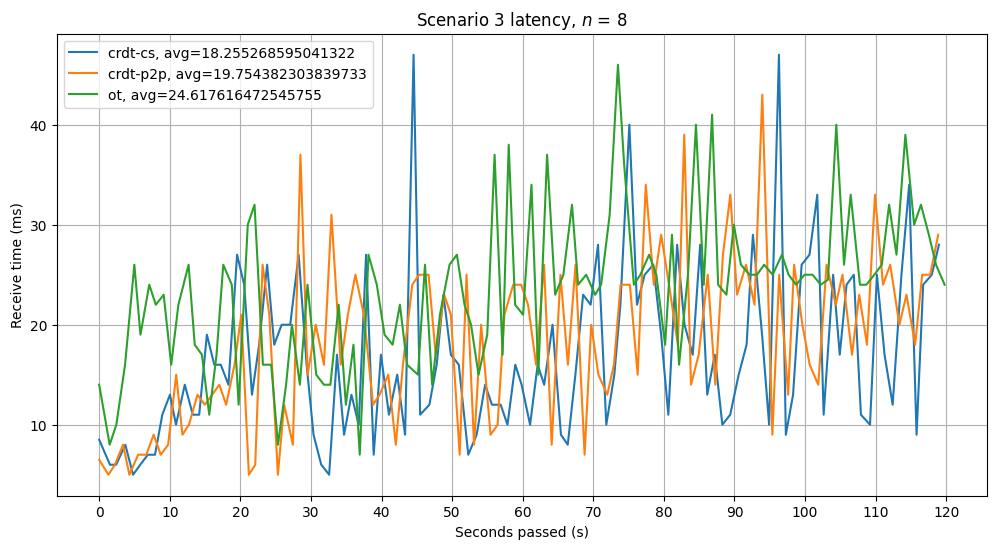
\includegraphics[width=15cm]{./assets/skripsi/benchmark-vis_cell_12_output_5}
 \caption{Grafik Waktu \textit{Resolve} Operasi Lokal pada Editor Setiap Variasi Aplikasi Pengguna PeerToCP}
 \label{fig:12-5}
\end{figure}

Latensi total diperoleh dari waktu penerapan operasi lokal dan nonlokal ditambah dengan waktu transmisi jaringan pada arsitektur yang berbeda-beda. Gambar~\ref{fig:7-5} menunjukkan perbedaan latensi yang cukup besar, serta lonjakan latensi yang terjadi beberapa kali sepanjang skenario ketiga berjalan. Hal ini dapat disebabkan oleh beberapa hal, yakni waktu \textit{resolve} operasi nonlokal dan adanya efek penumpukan \textit{update} yang diilustrasikan pada diagram gambar~\ref{diagram:snowball}.

\begin{figure}
 \centering
 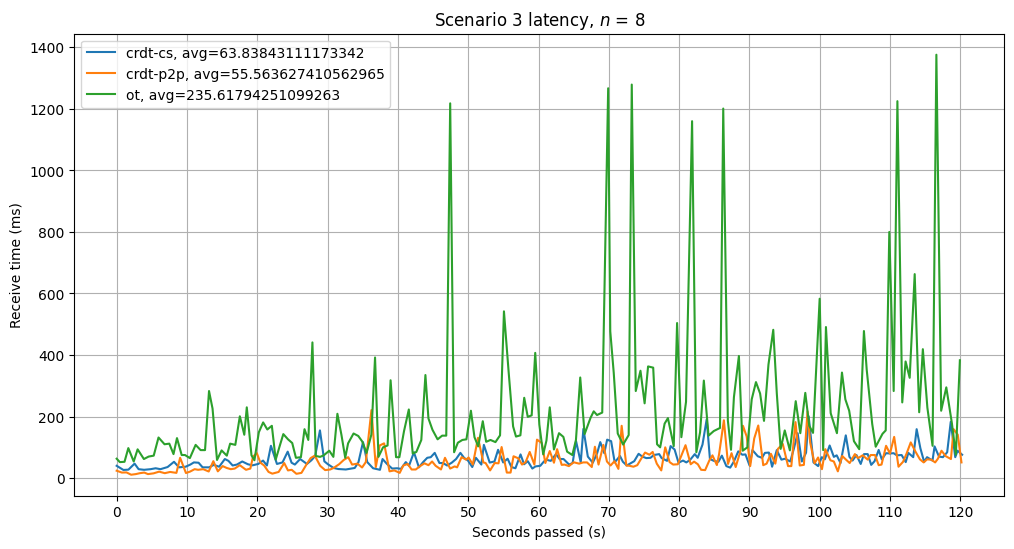
\includegraphics[width=15cm]{./assets/skripsi/benchmark-vis_cell_7_output_5}
 \caption{Grafik Mean Latensi pada Operasi Nonlokal Setiap Variasi Aplikasi Pengguna PeerToCP}
 \label{fig:7-5}
\end{figure}

\begin{figure}
 \centering
 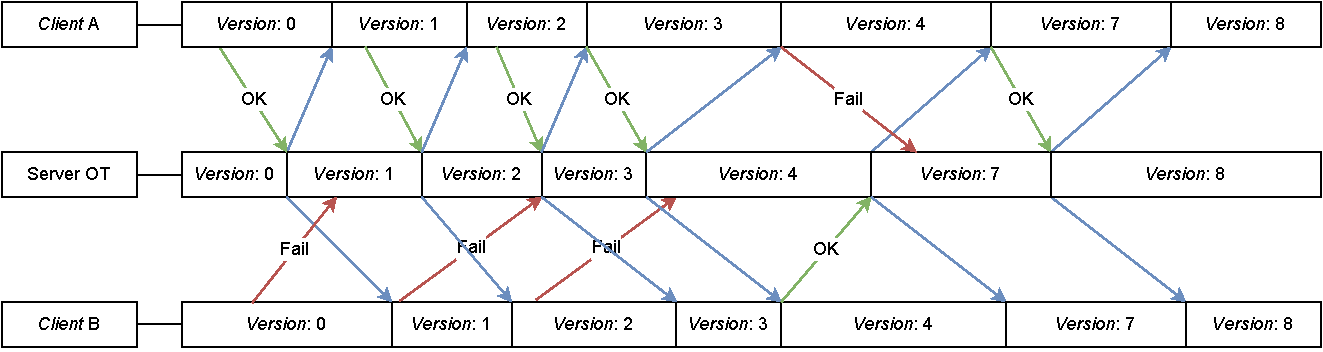
\includegraphics[width=15cm]{./assets/skripsi/Snowball}
 \caption{Diagram Ilustrasi Penumpukan \textit{Update}}
 \label{diagram:snowball}
\end{figure}

Pada arsitektur \textit{operational transformation} berbasis \textit{client-server}, \textit{update} dari suatu klien tidak akan diterima oleh server apabila klien tersebut belum memiliki versi terbaru dari server. Penumpukan \textit{update} ini dapat terjadi karena klien tersebut semakin tidak bisa mengirimkan datanya karena semakin besar dan selalu didahului oleh klien lain yang berada dalam jaringan tersebut. Penumpukan ini dapat menyebabkan tidak dapat diperbaruinya salah satu klien dan transmisi data keluar yang besar karena pengiriman \textit{update} besar yang dilakukan terus menerus.

Dalam praktis penggunaan realistisnya, hal ini diperkirakan tidak umum terjadi karena frekuensi pengetikan atau pemasukan karakter tidak dilakukan secara bersamaan dan tidak sebanyak skenario pertama dan kedua. Operasi salin dan tempel secara berkali-kali dapat berpotensi menyebabkan hal ini terjadi karena perubahan dokumen dalam jumlah karakter yang banyak terjadi. Namun dalam praktisnya, operasi tersebut diasumsikan hanya dilakukan dengan jeda frekuensi yang membolehkan setiap klien dalam jaringan memperbarui replikanya sebelum operasi besar lain dilakukan.

Skenario empat menguji latensi \textit{shell} yang dapat digunakan secara bersama. Secara umum, latensi tersebut dideskripsikan pada tabel~\ref{tab:latency-4}. Berbeda halnya dengan \textit{editor teks} yang waktu penerapan operasinya berdampak sebesar 20--70ms atau lebih. Struktur data berupa \textit{dictionary} sederhana pada \textit{shell} tidak memberikan perbedaan yang signifikan seperti yang digambarkan pada gambar grafik~\ref{fig:13-5}.

% Please add the following required packages to your document preamble:
% \usepackage{multirow}
\begin{table}[H]
 \centering
\begin{tabular}{|c|rrr|rrr|rrr|}
\hline
\multirow{2}{*}{$n$} & \multicolumn{3}{c|}{\textbf{CRDT Peer-To-Peer}} & \multicolumn{3}{c|}{\textbf{CRDT Client Server}} & \multicolumn{3}{c|}{\textbf{OT Client Server}} \\ \cline{2-10}
 & \multicolumn{1}{c|}{Mean} & \multicolumn{1}{c|}{Median} & \multicolumn{1}{c|}{Max} & \multicolumn{1}{c|}{Mean} & \multicolumn{1}{c|}{Median} & \multicolumn{1}{c|}{Max} & \multicolumn{1}{c|}{Mean} & \multicolumn{1}{c|}{Median} & \multicolumn{1}{c|}{Max} \\ \hline
\textbf{2} & \multicolumn{1}{r|}{3.05} & \multicolumn{1}{r|}{3.00} & 5.00 & \multicolumn{1}{r|}{16.75} & \multicolumn{1}{r|}{17.00} & 19.00 & \multicolumn{1}{r|}{31.79} & \multicolumn{1}{r|}{30.00} & 170.00 \\ \hline
\textbf{4} & \multicolumn{1}{r|}{3.13} & \multicolumn{1}{r|}{3.00} & 6.00 & \multicolumn{1}{r|}{16.55} & \multicolumn{1}{r|}{17.00} & 21.00 & \multicolumn{1}{r|}{44.47} & \multicolumn{1}{r|}{32.00} & 309.00 \\ \hline
\textbf{8} & \multicolumn{1}{r|}{3.36} & \multicolumn{1}{r|}{3.00} & 19.00 & \multicolumn{1}{r|}{17.16} & \multicolumn{1}{r|}{17.00} & 35.00 & \multicolumn{1}{r|}{59.86} & \multicolumn{1}{r|}{30.33} & 551.00 \\ \hline
\end{tabular}
 \caption{Statistik Latensi Operasi Nonlokal pada Skenario Keempat (\textit{Shell} Bersama) dalam Satuan ms}
 \label{tab:latency-4}
\end{table}

\begin{figure}
 \centering
 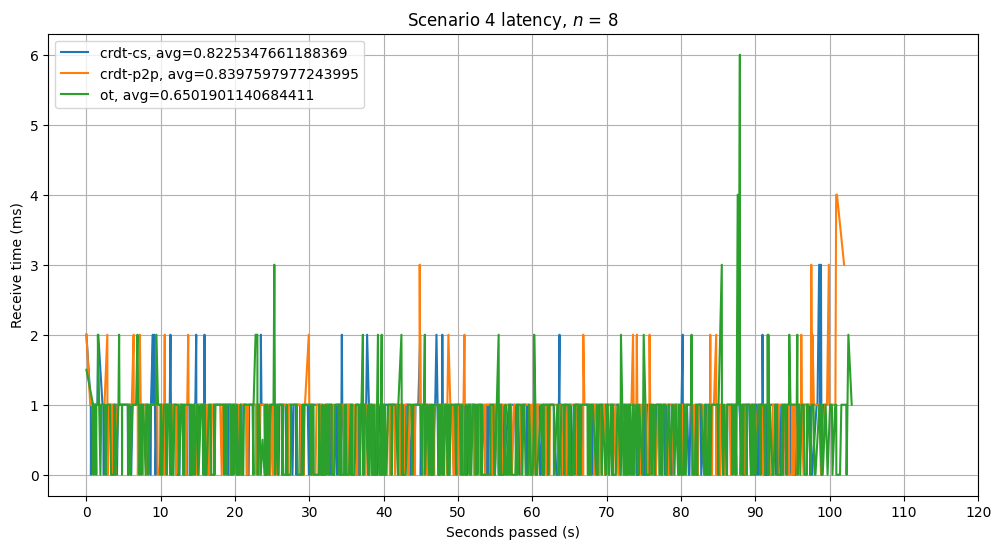
\includegraphics[width=15cm]{./assets/skripsi/benchmark-vis_cell_13_output_5}
 \caption{Grafik Waktu \textit{Resolve} Operasi Lokal pada \textit{Shell} Setiap Variasi Aplikasi Pengguna PeerToCP}
 \label{fig:13-5}
\end{figure}

Hal ini dikarenakan operasi penerapan dari \textit{append-only array} pada \textit{operational transformation} memiliki kompleksitas waktu konstan secara \textit{amortized}. Sehingga secara skalabilitas, hanya berpengaruh terhadap efektivitas dan performa latensi dari transmisi data, yang mengalami permasalahan sama seperti pada skenario pertama, kedua, dan ketiga seperti yang ditunjukkan pada gambar grafik~\ref{fig:9-5}. Faktor lain yang mempengaruhi alasan latensi \textit{operational transformation} lebih lambat dari pada CRDT \textit{client-server} ialah mekanisme komunikasinya. Implementasi CRDT Yjs dilengkapi dengan proses \textit{encoding} dan \textit{decoding} yang membuat transmisinya dalam jaringan untuk data yang besar dapat lebih cepat, serta tidak diperlukan adanya operasi \textit{update} yang dilakukan secara berurutan. Sementara implementasi variasi \textit{operational transformation}-nya masih menggunakan mekanisme \textit{update} yang sama dengan \textit{editor teks}-nya, hanya dengan perbedaan kompleksitas waktu \textit{update} konstan \textit{shell}.

\begin{figure}
 \centering
 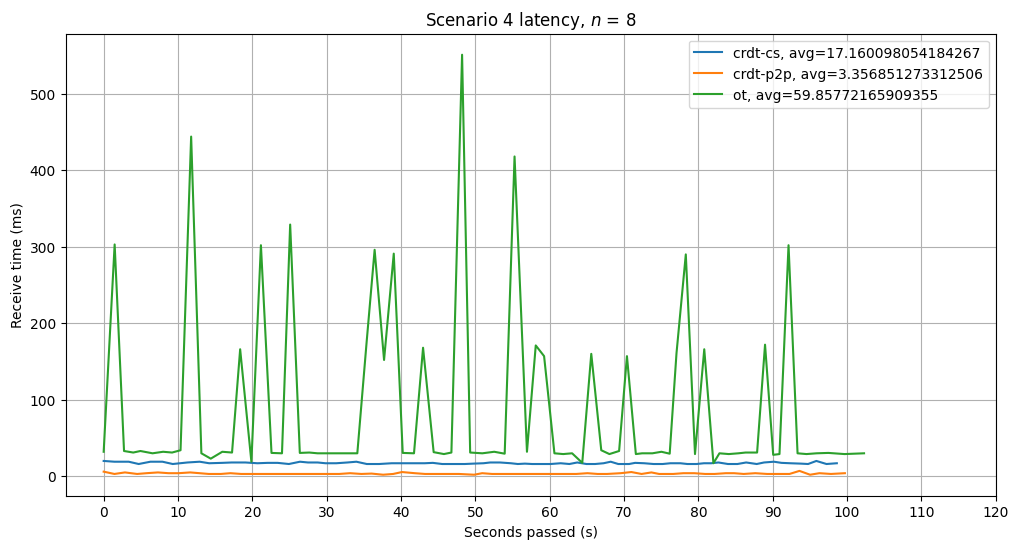
\includegraphics[width=15cm]{./assets/skripsi/benchmark-vis_cell_9_output_5}
 \caption{Grafik Mean Latensi pada Operasi Nonlokal Setiap Variasi Aplikasi Pengguna PeerToCP}
 \label{fig:9-5}
\end{figure}

Bila dibandingkan dengan arsitektur \textit{peer-to-peer}, setiap \textit{peers} dalam jaringan tersebut berada dalam jarak yang cenderung dekat. Latensinya akan lebih rendah dibandingkan kedua arsitektur \textit{client-server} yang harus melewati \textit{server} terlebih dahulu. Secara umum, variasi yang terbaik ialah variasi CRDT dengan arsitektur \textit{peer-to-peer} sejumlah $n$ tertentu. Dalam konteks eksperimen ini, untuk $n \leq 8$, variasi \textit{peer-to-peer} masih memberikan performa terbaik dari setiap variasi lainnya dari aspek \textit{responsiveness}. Diperkirakan untuk suatu nilai $n > 8$, atau jarak antar \textit{peers} yang lebih jauh, variasi CRDT dengan arsitektur \textit{client-server} dapat dipertimbangkan sebagai alternatif. Dalam beberapa kasus lainnya, CRDT \textit{peer-to-peer} dengan WebRTC dapat mengalami permasalahan antar \textit{peers} yang tidak dapat saling terhubung. Sehingga, alternatif berupa server penghubung, \textit{relay} atau STUN dapat digunakan dan latensinya memerlukan eksperimen lebih lanjut untuk dapat dibandingkan. Variasi \textit{operational transformation} juga dapat dipertimbangkan, karena secara teori operasi \textit{update}-nya yang konstan dapat memberikan latensi yang lebih baik karena memanfaatkan sifat \textit{append-only array} dan hanya satu \textit{peer} atau klien yang bertanggung jawab untuk meneruskan data interaksinya pada suatu \textit{shell}.

Untuk mendapatkan latensi yang optimal, struktur data CRDT dapat dimodifikasi dengan memanfaatkan sifat tersebut. Lebih lanjut, sistem dapat dimodifikasi untuk menentukan arsitektur optimal antara \textit{peer-to-peer} tanpa \textit{relay server} seperti pada eksperimen ini, \textit{peer-to-peer} dengan \textit{relay server} untuk menangani \textit{peer} yang tidak dapat terhubung oleh WebRTC, atau pun \textit{client-server} apabila banyaknya pengguna atau \textit{peer} dalam jaringan cukup banyak. Dari segi latensi, pertimbangan hal tersebut dapat ditentukan dengan metriks sederhana seperti \textit{ping} antar pengguna yang dilakukan dari layar belakang aplikasi. Namun, dalam praktisnya terdapat beberapa faktor lain yang harus dipertimbangkan, yakni berupa sifat \textit{lightweight} atau sebarapa banyak proses atau pekerjaan, serta memori yang harus disediakan oleh server dan penggunanya.

\section{Aspek \textit{Lightweight}}

Aspek ini memaparkan seberapa besar \textit{resource} komputasi yang dibutuhkan untuk setiap \textit{peers} dan servernya. Semua metriks RAM diukur dengan melakukan normalisasi ke nol sesaat sebelum uji kasus dimulai. Pengukuran ini didasarkan untuk membandingkan perubahan pertumbuhan. Selain itu, dalam beberapa kasus dalam menjalankan klien, aplikasi elektron yang berjalan di atas Chromium memiliki sistem \textit{garbage collection} dan \textit{cache}~\citep{chromium}. Sehingga, pengukuran skenario yang dilakukan relatif terhadap ukuran memori sesaat sebelum tes dimulai untuk memberikan perbandingan pertumbuhan yang lebih jelas. Pada mulanya, setiap server mulai dengan RAM yang relatif rendah, yakni di bawah 20MiB. Sementara setiap peers mulai dengan RAM yang cenderung lebih tinggi, yakni sekitar 200 MiB. Aplikasi ini membutuhkan memori yang cukup besar karena menggunakan \textit{framework} Electron yang menjalankan peramban web Chromium pada \textit{front-end}-nya.

\begin{table}[H]
 \centering

\begin{tabular}{|cc|r|r|r|}
\hline
\multicolumn{2}{|c|}{$n$} & \multicolumn{1}{c|}{\textbf{2}} & \multicolumn{1}{c|}{\textbf{4}} & \multicolumn{1}{c|}{\textbf{8}} \\ \hline
\multicolumn{1}{|c|}{\multirow{4}{*}{\textbf{CRDT Peer-To-Peer}}} & CPU & 39.1964893 & 60.13947488 & 62.2870496 \\ \cline{2-5}
\multicolumn{1}{|c|}{} & RAM & 16.57856816 & 19.24442935 & 21.30499303 \\ \cline{2-5}
\multicolumn{1}{|c|}{} & Net In & 28.5230253 & 96.16536701 & 229.4788353 \\ \cline{2-5}
\multicolumn{1}{|c|}{} & Net Out & -28.03809012 & -93.97903876 & -223.6266535 \\ \hline
\multicolumn{1}{|c|}{\multirow{4}{*}{\textbf{CRDT Client Server}}} & CPU & 33.96390498 & 57.38616741 & 56.89049428 \\ \cline{2-5}
\multicolumn{1}{|c|}{} & RAM & 14.92823532 & 19.12934751 & 20.94699478 \\ \cline{2-5}
\multicolumn{1}{|c|}{} & Net In & 19.46582482 & 27.68880062 & 30.96869733 \\ \cline{2-5}
\multicolumn{1}{|c|}{} & Net Out & -19.76281471 & -21.21326889 & -18.73440885 \\ \hline
\multicolumn{1}{|c|}{\multirow{4}{*}{\textbf{OT Client Server}}} & CPU & 47.79374975 & 73.29454876 & 65.25737338 \\ \cline{2-5}
\multicolumn{1}{|c|}{} & RAM & 25.9460194 & 31.17265199 & 36.33549154 \\ \cline{2-5}
\multicolumn{1}{|c|}{} & Net In & 62.24127487 & 99.81376692 & 87.42216719 \\ \cline{2-5}
\multicolumn{1}{|c|}{} & Net Out & -12962.04576 & -28872.47276 & -18344.14905 \\ \hline
\end{tabular}
 \label{tab:resource-client-1}
 \caption{Statistik Mean Aktivitas dan \textit{Resource} Aplikasi Pengguna pada Skenario Pertama}
\end{table}

Tabel~\ref{tab:resource-client-1} berturut-turut memiliki parameter yang menunjukkan aktivitas utilitasi CPU dalam satuan persen utilisasi, 100\% utilisasi berarti sistem menggunakan satu \textit{core} vCPU dengan penuh. Selanjutnya sumber daya atau resource RAM yang sudah dinormalisasi dalam satuan MiB, diikuti dengan kecepatan penerimaan dan pengiriman data dalam satuan kilobits per detik. Penggunaan RAM dan penerimaan data pada variasi CRDT \textit{peer-to-peer} cenderung lebih tinggi untuk $n = 8$, hal ini disebabkan karena pada variasi ini, semakin banyak \textit{peers} pada jaringan, berarti semakin banyak pula replika dokumen yang harus disinkronisasi. Karena \textit{signalling server} pada variasi ini tidak berperan dalam transmisi data CRDT, sehingga setiap \textit{peers} akan bertanggung jawab untuk saling memberikan informasi satu sama lain dalam memastikan kesamaan informasi pada setiap replikanya. Dari segi banyaknya data yang masuk ke dalam aplikasi variasi CRDT memastikan bahwa data-data tersebut dapat digunakan secara langsung dan setiap data yang dikirimkan akan digunakan tanpa ada kasus penolakan \textit{update} seperti pada variasi OT. Sehingga dari segi transmisi data keluar, variasi CRDT dianggap jauh lebih memenuhi aspek \textit{lightweight} dibandingkan variasi OT.

Variasi aplikasi CRDT \textit{client-server} secara relatif memberikan performa yang lebih baik untuk setiap variasi dari PeerToCP. Dari segi utilisasi CPU pada \textit{environment} pengujian dengan dua core vCPU (utilisasi maksimal 200\%), skenario pertama dengan $n \geq 4$ secara rata-rata hanya menggunakan sekitar 1/3 \textit{resource} dari CPU seperti yang terlihat pada grafik gambar~\ref{fig:2-19}. Metriks ini dapat dipertimbangkan dengan tambahan bahwa skenario ini memberikan muatan operasi-operasi yang relatif lebih besar dan banyak dari perkiraan aktivitas penggunaan normal. Selain itu, sistem operasi secara optimal akan menentukan proses yang harus diutamakan baik dari segi penyimpanan dan prioritas komputasi saat berjalannya aplikasi-aplikasi di atas sistem.

\begin{figure}
 \centering
 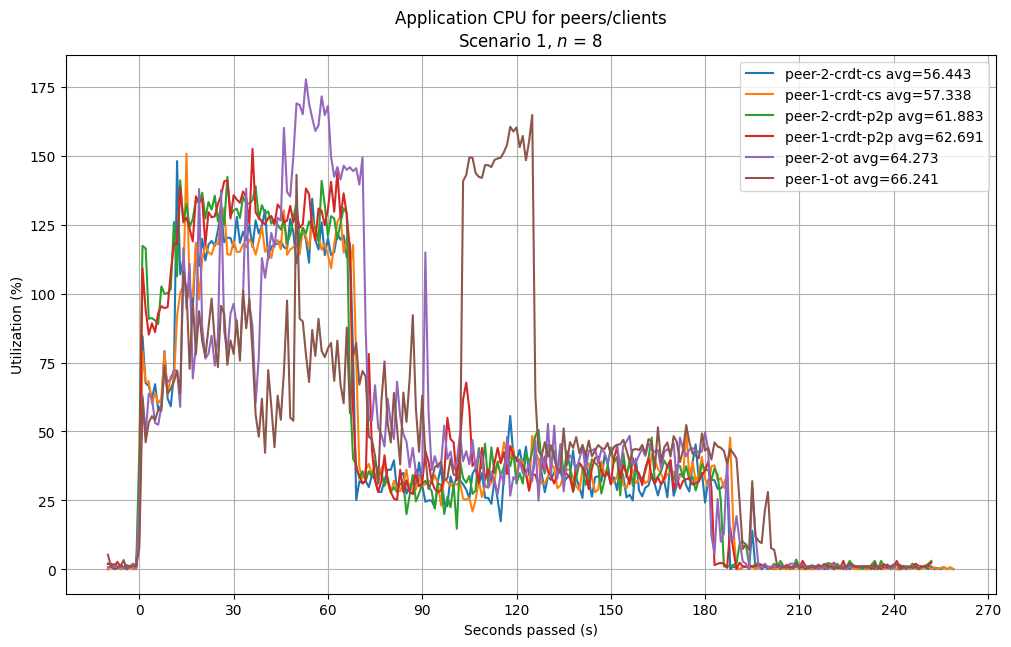
\includegraphics[width=13cm]{./assets/skripsi/benchmark-vis_cell_2_output_19}
 \caption{Grafik Perbandingan Utilisasi CPU pada Klien Pertama dan Klien Kedua untuk $n = 8$}
 \label{fig:2-19}
\end{figure}

\begin{figure}
 \centering
 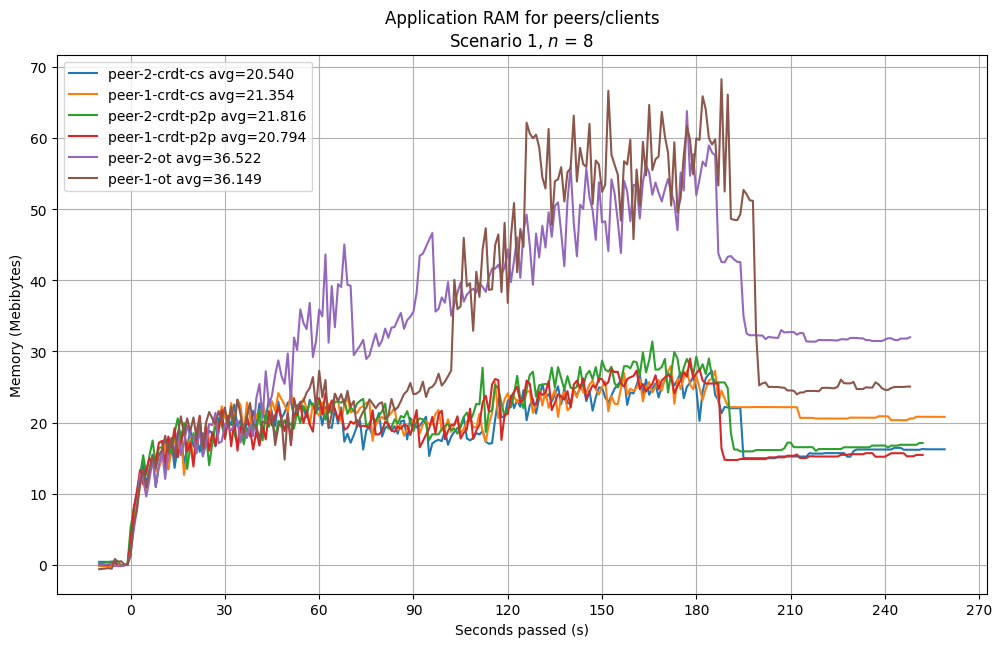
\includegraphics[width=13cm]{./assets/skripsi/benchmark-vis_cell_2_output_21}
 \caption{Grafik Perbandingan Penggunaan RAM pada Klien Pertama dan Klien Kedua untuk $n = 8$}
 \label{fig:2-21}
\end{figure}

Dari segi memori, kedua variasi CRDT memberikan pertumbuhan yang lebih optimal dibandingkan variasi OT. Namun, setiap variasinya menggunakan memori yang relatif kecil terhadap kapasitas penuh perangkat \textit{environment} pengujian, yakni sekitar 15\%. Penggunaan memori sebelum dinormalisasi rata-rata dimulai dengan menggunakan sekitar 200MiB, diikuti dengan pertumbuhan penggunaan seperti yang terlihat pada grafik gambar~\ref{fig:2-21}. Sistem operasi dapat memanfaatkan CPU dan RAM yang \textit{idle} sehingga utilisasinya dapat mendominasi proses lain pada komputer. Selama aplikasi tidak menggunakan utilisasi penuh yang mengganggu jalannya aktivitas pengguna dalam berinteraksi dengan aplikasi PeerToCP dan aplikasi lain, maka penggunaannya untuk jumlah pengguna yang terbatas dan diuji dalam eksperimen bagi pengguna setiap variasi PeerToCP dianggap memenuhi aspek \textit{lightweight} dari segi utilisasi CPU dan RAM.


\begin{table}[H]
 \centering
\begin{tabular}{|cc|r|r|r|}
\hline
\multicolumn{2}{|c|}{$\boldsymbol{n}$} & \multicolumn{1}{c|}{\textbf{2}} & \multicolumn{1}{c|}{\textbf{4}} & \multicolumn{1}{c|}{\textbf{8}} \\ \hline
\multicolumn{1}{|c|}{\multirow{4}{*}{\textbf{CRDT Peer-To-Peer}}} & CPU & 0.01 & 0.02 & 0.10 \\ \cline{2-5}
\multicolumn{1}{|c|}{} & RAM & 0.67 & -0.03 & 0.40 \\ \cline{2-5}
\multicolumn{1}{|c|}{} & Net In & 10.72 & 14.81 & 60.72 \\ \cline{2-5}
\multicolumn{1}{|c|}{} & Net Out & -10.24 & -15.79 & -83.11 \\ \hline
\multicolumn{1}{|c|}{\multirow{4}{*}{\textbf{CRDT Client Server}}} & CPU & 0.93 & 1.29 & 1.68 \\ \cline{2-5}
\multicolumn{1}{|c|}{} & RAM & 5.01 & 6.83 & 9.54 \\ \cline{2-5}
\multicolumn{1}{|c|}{} & Net In & 73.26 & 176.64 & 324.19 \\ \cline{2-5}
\multicolumn{1}{|c|}{} & Net Out & -71.79 & -193.90 & -391.66 \\ \hline
\multicolumn{1}{|c|}{\multirow{4}{*}{\textbf{OT Client Server}}} & CPU & 4.85 & 14.18 & 24.33 \\ \cline{2-5}
\multicolumn{1}{|c|}{} & RAM & 30.92 & 41.88 & 69.99 \\ \cline{2-5}
\multicolumn{1}{|c|}{} & Net In & 52318.08 & 167768.04 & 308540.87 \\ \cline{2-5}
\multicolumn{1}{|c|}{} & Net Out & -26494.76 & -84932.31 & -156178.28 \\ \hline
\end{tabular}
 \caption{Statistik Mean Aktivitas dan \textit{Resource Server} pada Skenario Pertama}
 \label{tab:resource-server-1}
\end{table}

Aspek \textit{lightweight} lainnya yang perlu dipertimbangkan ialah penggunaan \textit{resource} atau sumber daya pada server yang dideskripsikan pada tabel~\ref{tab:resource-server-1}. Server CRDT \textit{peer-to-peer} yang akan menyelesaikan \textit{signalling} WebRTC menggunakan \textit{resource} RAM dan CPU yang sangat minim, dan secara teori tidak mengalami perbedaan signifikan untuk suatu jaringan yang sedang menggunakan aplikasi ini, karena hanya menangani klien yang akan masuk dan keluar pada suatu kelompok \textit{peer}. Berbeda halnya dengan arsitektur \textit{client-server}, selain berperan dalam memelihara koneksi kelompok klien dalam suatu ruangan, server juga akan memelihara kondisi replika pada setiap klien dalam jaringan. Dalam beberapa referensi implementasi, penyimpanan dokumen dapat memerlukan basis data yang lebih besar untuk dapat menampung lebih banyak data pada kelompok jaringan. Dalam eksperimen ini, basis data pada setiap variasi tidak menggunakan teknologi pihak ketiga dan hanya menggunakan struktur data bawaan sederhana pada server.

Dari data statistik tersebut, \textit{drawback} dari transmisi minimal pada aplikasi pengguna CRDT \textit{client-server} ialah transmisi yang lebih besar dari sisi server, dan sebaliknya pada CRDT \textit{peer-to-peer}, transmisi data cenderung lebih kecil dibandingkan dengan variasi \textit{peer-to-peer}nya. Variasi OT memiliki muatan paling besar dibandingkan dengan variasi lain yang juga secara tidak langsung memengaruhi utilisasi \textit{resource}-nya menyesuaikan untuk menangani permintaan transmisi data masuk dan keluar yang cenderung lebih banyak. Dari aspek \textit{lightweight}, arsitektur \textit{client-server} pada OT tidak dipreferensi penggunaannya dan membutuhkan tinjauan kembali untuk dioptimisasi protokol pengiriman data atau pemanfaatan variasi algoritma OT yang lebih kompleks dan optimal untuk dapat menangani skenario muatan di atas rata-rata seperti skenario pertama.

\section{Evaluasi Latensi}





\section{Evaluasi Performa}